% ==========================================
% BÖLÜM 4.6: MOD_UI_VIEW (ARAYÜZ ÇİZİM VE RENDER KATMANI)
% ==========================================

\newpage
\section{\texttt{mod\_UI\_View}}

\texttt{mod\_UI\_View}, uygulamanın Grafik Kullanıcı Arayüzü (GUI) bileşenlerinin çalışma zamanında (\textit{Runtime}) dinamik olarak inşasından, görsel nesne parametrelerinin yapılandırılmasından ve hesaplanan verilerin ekran elemanlarına aktarılmasından (\textit{Rendering}) sorumlu Görünüm Katmanı (\textit{View Layer}) modülüdür.

Uygulamada standart \texttt{UserForm} yapısı yerine, \texttt{Worksheet} üzerine gömülen asenkron OLE Panelleri (\texttt{MSForms.Frame}) tercih edilmiştir. Bu mimari yaklaşımda \texttt{mod\_UI\_View}, arayüzün nesnel tasarım kalıplarına uygun şekilde soyutlanmasını sağlar. İş mantığı katmanı (\texttt{mod\_Services}) ile kullanıcı etkileşim katmanı (\texttt{mod\_UI\_Events}) arasında köprü kurarak, ham veriyi görsel tablolara (\texttt{ListBox}) dökme işlevini üstlenir.

Modülün temel tasarım ve mimari sorumlulukları üç ana grupta toplanmaktadır:

\begin{itemize}\setlength{\itemsep}{0pt}\setlength{\parskip}{1pt}
    \item \textbf{Dinamik Kontrol Oluşturma (UI Builder):} Çalışma sayfasına eklenecek \texttt{Frame}, \texttt{CommandButton}, \texttt{ListBox}, \texttt{Label}, \texttt{TextBox} ve \texttt{ComboBox} gibi nesnelerin koordinat, boyut, renk ve varsayılan durumlarını programatik olarak tanımlar.
    \item \textbf{Veri Bağlama ve Görselleştirme (Data Rendering):} Servis katmanından dönen dizileri ve koleksiyonları dinamik listelere yükler; hata durumlarında kullanıcıya durum göstergeleri (\texttt{OK}, \texttt{HATA}) sunar.
    \item \textbf{Olay Dinleyici Kaydı (Event Registration):} Çizilen her bir dinamik butonu, tıklama olaylarının yakalanabilmesi amacıyla merkezi \texttt{ButtonCollection} koleksiyonuna bağlar.
\end{itemize}

\vspace{0.15cm}

\begin{infobox}{\faPalette\ Arayüz Bileşenleri ve Modüler Yapı}
Görsel katmanda yer alan tüm panel oluşturma (\texttt{Create*}) ve veri işleme (\texttt{Render*}) Prosedürleri, \texttt{mod\_Config} modülündeki merkezi sabitleri (\texttt{PANEL\_WIDTH}, \texttt{COLOR\_GREEN} vb.) referans alır. Bu sayede arayüz tasarımındaki renk ve boyut değişiklikleri kod tekrarı olmadan tek bir noktadan yönetilebilir.
\end{infobox}

\vspace{0.3cm}

\textbf{\textcolor{primary}{1. Geliştirme Ortamı ve Modül Yapısı}}

Aşağıdaki ekran görüntüsünde, VBA Geliştirme Ortamı (\textit{VBE}) üzerinde \texttt{mod\_UI\_View} modülünün barındırdığı yapıcı, yardımcı ve render prosedürlerinin genel listesi sunulmaktadır:

\vspace{0.3cm}

\begin{figure}[htbp]
    \centering
    \fboxsep=0pt
    \fboxrule=0.8pt
    \fcolorbox{bordergray}{white}{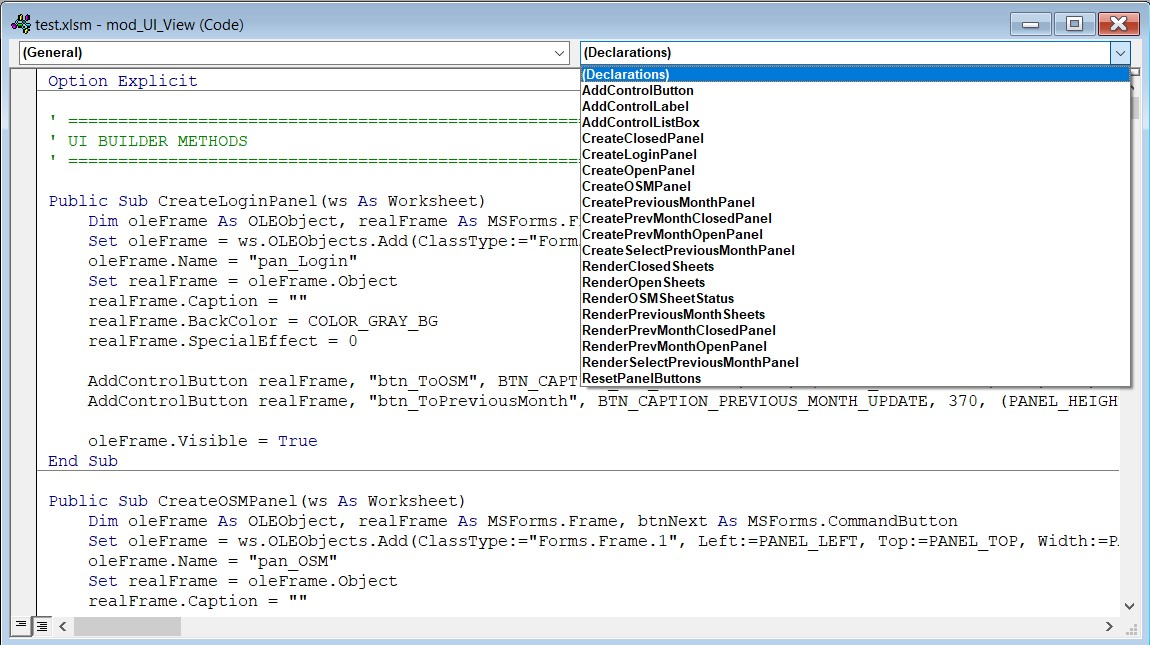
\includegraphics[width=0.88\textwidth, keepaspectratio]{mod_UI_View.jpg}}
    \caption{\texttt{mod\_UI\_View} Modülü Prosedür ve Fonksiyon Dizilimi}
    \label{fig:mod_ui_view_code}
\end{figure}

\vspace{0.2cm}

\textbf{\textcolor{primary}{2. Arayüz Oluşturucuları (UI Builder Methods)}}

Çalışma kitabı ilk açıldığında veya yapılandırma sıfırlandığında, sistemdeki her bir iş akışı paneli (\texttt{Login}, \texttt{OSM}, \texttt{Open}, \texttt{Closed}, \texttt{PreviousMonth}, \texttt{SelectPreviousMonth} vb.) özel oluşturucu prosedürler tarafından inşa edilir. 

Panel yapım aşamasında izlenen standart işlem adımları şunlardır:
\begin{enumerate}\setlength{\itemsep}{0pt}\setlength{\parskip}{1pt}
    \item Aktif sayfada \texttt{OLEObjects.Add} fonksiyonu ile yeni bir \texttt{MSForms.Frame} örneği açılır.
    \item Panelin arka plan rengi, kenarlık stili ve konum parametreleri ayarlanır.
    \item Yardımcı private metotlar (\texttt{AddControlButton}, \texttt{AddControlLabel}, \texttt{AddControlListBox}) kullanılarak panel içerisine gerekli kontrol elemanları yerleştirilir.
    \item Oluşturulan buton referansları bellek kaybolmasını önlemek için \texttt{clsDynamicButton} wrapper sınıfına tescil edilir.
\end{enumerate}

\vspace{0.3cm}

\textbf{\textcolor{primary}{3. Veri Render Yöneticileri (UI Renderer Methods)}}

Kullanıcı paneller arasında geçiş yaptığında veya tarama/güncelleme butonlarına bastığında \texttt{Render*} prosedürleri devreye girer. Bu prosedürler, arka plandaki servislerden dönen dinamik veriyi okur ve \texttt{ListBox} elemanlarını kolon genişliklerine göre biçimlendirerek doldurur.

\newpage
Render sürecinde öne çıkan temel mantıksal mekanizmalar:
\begin{itemize}\setlength{\itemsep}{0pt}\setlength{\parskip}{1pt}
    \item \textbf{Sütun Başlıkları ve Tablo Hizalama:} Her render işleminde \texttt{ListBox.Clear} ile liste sıfırlanır ve ilk satıra sabit tablo başlıkları yüklenir.
    \item \textbf{Otomatik Veri Dönüşümü ve Eşleme:} Veritabanı hücre adresleri (\texttt{D4}, \texttt{K2} vb.) ve ilişkili sayfa isimleri birleştirilerek açıklayıcı metinler (\textit{Örn: D4 (ARIZA)}) halinde listeye aktarılır.
    \item \textbf{Zamanlayıcı ve Otomatik Kilit Mekanizması:} Ekran render edildikten sonra tarama butonlarının aktif kalması ve hatalı çift tıklamaların önlenmesi amacıyla \texttt{Application.OnTime} kullanılarak panel belirli bir süre sonra otomatik kilit durumuna alınır.
    \item \textbf{Boş Satır Tamamlama (Dikey Izgara Düzeni):} Görsel bütünlüğü korumak amacıyla veriler yüklendikten sonra \texttt{ListBox} dikey boyutu dolana kadar boş satır tamamlama döngüsü (\texttt{Do While ListCount < 12}) çalıştırılır.
\end{itemize}

\vspace{0.15cm}

\begin{warningbox}{\faExclamationTriangle\ Arayüz Kararlılığı ve Hata İşleme}
Render işlemleri esnasında geçersiz sayfa yapıları veya silinmiş OLE nesneleri nedeniyle çökme yaşanmaması adına, buton sıfırlayıcı yardımcı prosedürlerde (\texttt{ResetPanelButtons}) yerel hata yönetimi (\texttt{On Error Resume Next}) uygulanmaktadır.
\end{warningbox}

\vspace{0.4cm}

\begin{tcolorbox}[colback=yellow!15,colframe=orange!80!black,leftrule=3.5pt,boxrule=0.4pt,top=5pt,bottom=5pt]
    \textbf{\textcolor{orange!80!black}{\faInfoCircle\ mod\_UI\_View Genel Özet ve Mimari Rolü:}}\\
    \small \texttt{mod\_UI\_View}, uygulamanın tüm görsel bileşenlerini ve tablo ekranlarını kod üzerinden dinamik üreten bir **Grafik Motoru** işlevi görür. Veri işleme mantığını görsel tasarımdan tamamen ayırarak (MVC mimari yaklaşımı), projenin sürdürülebilirliğine ve kolay genişletilebilir bir arayüz yapısına kavuşmasına doğrudan katkı sağlar.
\end{tcolorbox}

\newpage

% ==========================================
% BÖLÜM 4.7: MOD_SERVICES (İŞ MANTIĞI VE VERİ SERVİSLERİ KATMANI)
% ==========================================

\section{\texttt{mod\_Services}}

\texttt{mod\_Services}, uygulamanın tüm veri işleme, hesaplama, veritabanı kesişim adresi bulma, sayfa tarama ve Excel hücre yazma algoritmalarından sorumlu **İş Mantığı Katmanıdır (Business Logic Layer)**. 

Arayüz katmanları (\texttt{mod\_UI\_View}, \texttt{mod\_UI\_Events}) kullanıcı etkileşimlerini yönetip form verilerini toplarken, \texttt{mod\_Services} arka planda verinin doğruluğunu denetler, metrikleri hesaplar ve veritabanı kesişim adreslerine güvenli yazma operasyonlarını yürütür.

Modül içerisinde yüksek işlem performansı ön planda tutulmuştur. Sayfalarda tek tek hücre okumak yerine, veriler belleğe dinamik diziler (\textit{Variant Arrays}) ve hızlı erişimli Sözlük nesneleri (\textit{Scripting.Dictionary}) olarak alınarak işlenir.

Modülün temel fonksiyonel sorumlulukları dört ana kategoride toplanmaktadır:

\begin{itemize}\setlength{\itemsep}{0pt}\setlength{\parskip}{1pt}
    \item \textbf{Çalışma Kitabı ve Sayfa Taramaları:} Kitap içerisindeki tüm sayfaları dolaşarak aktif vaka veya bakım raporlarını tespit eder (\texttt{ScanWorkbookSheets}, \texttt{ScanPreviousMonthSheets}).
    \item \textbf{Tarih ve Dinamik Adres Algoritmaları:} Rapor tarihlerini analiz eder, hedef veritabanı sayfasında ilgili tarih kolonu ile durum satırının kesiştiği hücreyi bulur (\texttt{GetReportDate}, \texttt{FindIntersectCell}).
    \item \textbf{Gelişmiş Metrik Hesaplamaları:} Personel bazlı kapalı vaka sayılarını ve geçmiş ay verilerini dinamik matrislerle hesaplar (\texttt{GetOpenCasesCalculated}, \texttt{GetClosedCasesCalculated}).
    \item \textbf{Veritabanı Yazma Motoru:} Arayüzdeki listelerden gelen verileri süzerek doğrudan veritabanı hücrelerine işler (\texttt{ExecuteDatabaseWrite}, \texttt{ExecutePreviousMonthWrite}).
\end{itemize}

\vspace{0.15cm}

\begin{infobox}{\faCogs\ Performans Odaklı Bellek Yönetimi (In-Memory Data Engine)}
\texttt{CountClosedCasesByPerson} ve \texttt{CountOpenCasesByPerson} gibi fonksiyonlar, çalışma sayfasındaki verileri \texttt{ws.Range.Value} komutuyla tek hamlede RAM üzerindeki çift boyutlu dizilere aktarır. Döngüler bellekte döndüğü için binlerce satırlık veriler milisaniyeler içerisinde işlenir.
\end{infobox}

\vspace{0.3cm}

\textbf{\textcolor{primary}{1. Geliştirme Ortamı ve Modül Yapısı}}

Aşağıdaki ekran görüntüsünde, VBA Geliştirme Ortamı (\textit{VBE}) üzerinde \texttt{mod\_Services} modülünün barındırdığı iş mantığı, tarama, hesaplama ve yardımcı fonksiyonların genel dizilimi gösterilmektedir:

\vspace{0.25cm}

% Resmin Tam Buraya Çakılması İçin Ortamsız Yapı
\begin{center}
    \fboxsep=0pt
    \fboxrule=0.8pt
    \fcolorbox{bordergray}{white}{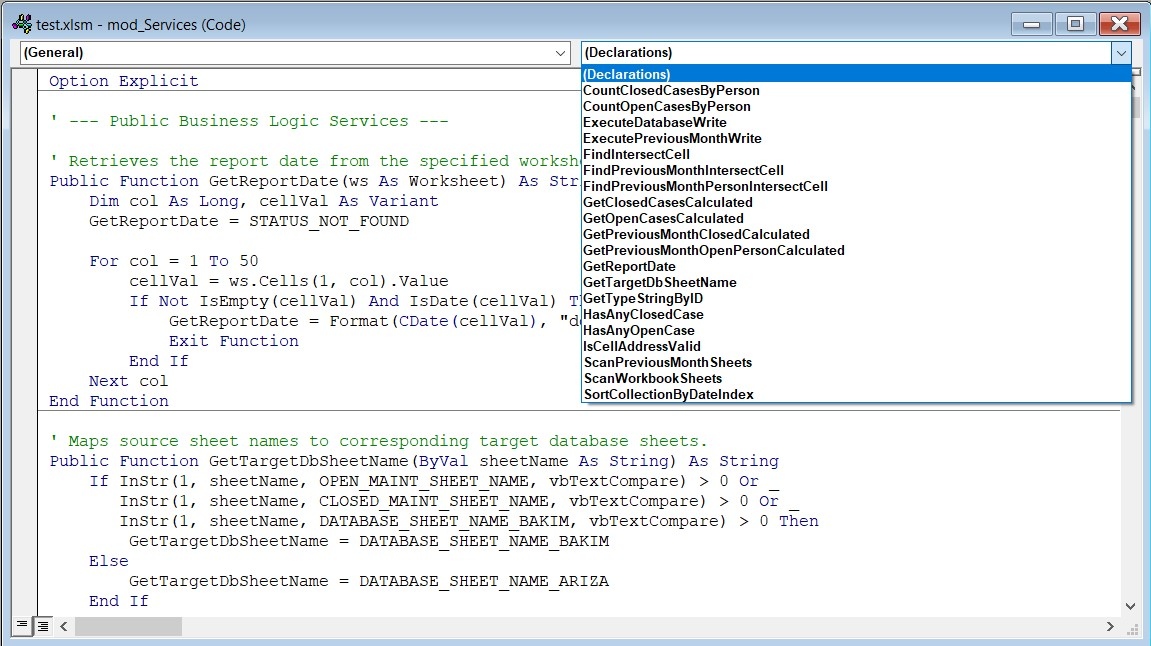
\includegraphics[width=0.85\textwidth, keepaspectratio]{mod_Services.jpg}}
    \captionof{figure}{\texttt{mod\_Services} Modülü Prosedür ve Fonksiyon Dizilimi}
    \label{fig:mod_services_code}
\end{center}

\vspace{0.25cm}

\textbf{\textcolor{primary}{2. Kesişim Adresi Algoritması (FindIntersectCell)}}

Veritabanı sayfalarında aranan tarihe ait sütun ile ilgili durum satırının kesiştiği hücre adresini (\textit{Örn: D4}) dinamik olarak tespit eden temel algoritma aşağıdadır:

\begin{lstlisting}[caption={Dinamik Kesişim Adresi Bulma Fonksiyonu}]
Public Function FindIntersectCell(ByVal dbSheetName As String, ByVal targetDateStr As String, ByVal searchColName As String, ByVal contextText As String) As String
    Dim dbWs As Worksheet, i As Long, tRow As Long, tCol As Long
    FindIntersectCell = STATUS_NOT_FOUND
    
    On Error Resume Next
    Set dbWs = ThisWorkbook.Sheets(dbSheetName)
    On Error GoTo 0
    If dbWs Is Nothing Or Not IsDate(targetDateStr) Then Exit Function
    
    ' 1. Tarih Sutununu Bul
    For i = dbWs.Columns(DB_OSM_DATES_START_COL).Column To dbWs.Columns(DB_OSM_DATES_END_COL).Column
        If IsDate(dbWs.Cells(1, i).Value) Then
            If CDate(dbWs.Cells(1, i).Value) = CDate(targetDateStr) Then tCol = i: Exit For
        End If
    Next i
    
    ' 2. Baglam Satirini Bul (searchColName uzerinde contextText aranir)
    ' . . . (dbLastRow hesaplanarak tRow indeksi tespit edilir)
    
    ' 3. Kesisim Adresini Dondur (Orn: "D4")
    If tRow > 0 And tCol > 0 Then
        FindIntersectCell = dbWs.Cells(tRow, tCol).Address(RowAbsolute:=False, ColumnAbsolute:=False)
    End If
End Function
\end{lstlisting}

\vspace{0.3cm}

\textbf{\textcolor{primary}{3. Personel Bazlı Gruplama ve Hesaplama Metotları}}

Sayfalardaki kapalı vakaları personellere göre gruplarken \texttt{Scripting.Dictionary} yapısı kullanılır. Sayılan değerler \texttt{FindIntersectCell} ile bulunan adreslerle birleştirilerek koleksiyona yüklenir:

\begin{lstlisting}[caption={Kapalı Vakaların Personel Bazlı Hesaplama Mimarisi}]
Public Function GetClosedCasesCalculated() As Collection
    Dim closedCol As New Collection, dict As Object, item As Variant
    Set dict = CreateObject("Scripting.Dictionary")
    
    For Each item In ScanWorkbookSheets()
        If (item(1) = RPT_TYPE_CLOSED_CASE Or item(1) = RPT_TYPE_CLOSED_MAINT) And item(2) <> STATUS_NOT_FOUND Then
            ' Kesisim adresi ile verileri birlestirip koleksiyona ekleme
            dbName = GetTargetDbSheetName(CStr(item(4)))
            For Each key In dict.Keys
                targetCell = FindIntersectCell(dbName, CStr(item(3)), DB_CLOSED_NAME_COL, CStr(key))
                If targetCell <> STATUS_NOT_FOUND And targetCell <> STATUS_NO_DB_SHEET Then
                    closedCol.Add Array(item(4), item(2), item(3), CStr(key), dict(key), targetCell)
                End If
            Next key
            dict.RemoveAll
        End If
    Next item
    Set GetClosedCasesCalculated = SortCollectionByDateIndex(closedCol, 3)
End Function
\end{lstlisting}

\vspace{0.3cm}

\textbf{\textcolor{primary}{4. Güvenli Veritabanı Yazma Motoru}}

Arayüzdeki listelerden okunan güncellenmiş değerler, parantezli sayfa eklerinden (\textit{Örn: D4 (ARIZA)}) ayıklanarak doğrudan veritabanı hücrelerine işlenir:

\begin{lstlisting}[caption={Veritabanı Hücre Yazma Operasyonu}]
Public Function ExecuteDatabaseWrite(lst As MSForms.ListBox, cellColIdx As Long, valColIdx As Long, sheetNameColIdx As Long) As Boolean
    Dim dbWs As Worksheet, i As Long, addr As String, caseVal As Long
    
    For i = 1 To lst.ListCount - 1
        addr = Trim("" & lst.List(i, cellColIdx))
        If InStr(addr, "(") > 0 Then addr = Trim(Split(addr, "(")(0))
        
        If addr <> "" And addr <> STATUS_NOT_FOUND And addr <> STATUS_NO_DB_SHEET Then
            targetDbName = GetTargetDbSheetName(Trim("" & lst.List(i, sheetNameColIdx)))
            Set dbWs = ThisWorkbook.Sheets(targetDbName)
            
            If Not dbWs Is Nothing Then
                caseVal = Val("" & lst.List(i, valColIdx))
                dbWs.Range(addr).Value = caseVal
            End If
        End If
    Next i
    ExecuteDatabaseWrite = True
End Function
\end{lstlisting}

\vspace{0.15cm}

\begin{warningbox}{\faExclamationTriangle\ Hata Önleme ve Hücre Doğrulama}
Yazma operasyonları öncesinde \texttt{IsCellAddressValid} fonksiyonu çalıştırılarak hücre adresinin varlığı teyit edilir. Olası sayfa bulunamama veya hatalı adres durumlarında yazma işlemi iptal edilerek kullanıcı bilgilendirilir.
\end{warningbox}

\vspace{0.4cm}

\begin{tcolorbox}[colback=yellow!15,colframe=orange!80!black,leftrule=3.5pt,boxrule=0.4pt,top=5pt,bottom=5pt]
    \textbf{\textcolor{orange!80!black}{\faInfoCircle\ mod\_Services Genel Özet ve Mimari Rolü:}}\\
    \small \texttt{mod\_Services}, uygulamanın **Çekirdek Veri Motorudur**. Arayüz bileşenlerinden bağımsız çalışır, girdi verilerini dönüştürür, dinamik adres kesişimlerini hesaplar ve Excel hücre düzeyindeki yazma/okuma operasyonlarını yüksek performansla gerçekleştirir.
\end{tcolorbox}